\documentclass[12pt]{article}
\usepackage{calc}
\usepackage{forloop}
\usepackage{xcolor}
\usepackage{tikz}
\usepackage[OT1]{fontenc}
\renewcommand*\familydefault{\sfdefault}
\usepackage{lstcustom}
\usepackage{tikz-uml}
\usepackage[absolute,overlay]{textpos}
\date{}

\lstdefinestyle{eclipseNoBox}{
  basicstyle={\small\lstfontfamily},
  emphstyle=\bfseries,
  keywordstyle=\color{keywordColor}\bfseries,
  commentstyle=\markupComments,
  stringstyle=\color{stringColor},
  numberstyle=\color{lineNumberColor}\lstfontfamily,
  morecomment=[s][\markupJavadocs]{/**}{*/}, % For Javadoc style comments
  showstringspaces=false,
  numbers=none,
}

\lstset{
  language=C++,
  style=eclipseNoBox,
  escapechar=\$
}
\newcommand*\circled[1]{\tikz[baseline=(char.base)]{
            \node[shape=circle,draw,inner sep=2pt] (char) {#1};}}

\usetikzlibrary{
    fit,
    calc,
    shadows,
    shapes.multipart,
    chains,
    arrows,
    snakes
}

\begin{document}

\begin{tikzpicture}[
    overlay,
    remember picture,
    list/.style={
        draw
        },
    >=stealth,
    start chain,
    xshift=-3cm
]
    \node[list,on chain] (A) {$A$};
    \node[list,on chain] (B) {$A/{\rm Rad}(A)$};
    \node[list,on chain] (C) {${\color{blue}L_1}\oplus {\color{blue}L_2}\oplus\cdots\oplus{\color{red}{L_n}}$};
    \node[list,on chain] (D) {${\color{blue}A_1}\oplus\cdots\oplus{\color{red} A_m}$};
    \node[list,on chain] (E) {${\color{blue}{\rm Mat}_{n_1}(D_1)}\oplus\cdots\oplus{\color{red} {\rm Mat}_{n_m}(D_m)}$};
    \node [align=center, anchor=north,yshift=-.5cm] at (A.south) (t0) {$A$ left Artinian};
    \node [align=center, anchor=south,yshift=.5cm] at (B.north) (t1) {Quotient by maximal nilpotent ideal\\ ${\rm Rad}(A)$ to get a semisimple ring};
    \node [align=center, anchor=north,yshift=-.5cm] at (C.south) (t2) {Decompose into direct sum\\ of minimal left ideals};
    \node [align=center, anchor=south,yshift=.5cm] at (D.north) (t3) {Group isomorphic entries\\ into simple components};
    \node [align=center, anchor=north,yshift=-.5cm] at (E.south) (t4) {Each component is a matrix ring over a\\ division ring, ${\rm Mat}_{n_i}(D_i)\cong n_iL$ consists of\\ $n_i$ copies of the same minimal left ideal};
    \draw [->] (A) -- (B) node (m1) [midway] {};
    \draw [->] (B) -- (C) node (m2) [midway] {};
    \draw [->] (C) -- (D) node (m3) [midway] {};
    \draw [->] (D) -- (E) node (m4) [midway] {};
    \draw [->] (t0) -- (A);
    \draw [->] (t1) -- (B);
    \draw [->] (t2) -- (C);
    \draw [->] (t3) -- (D);
    \draw [->] (t4) -- (E);
    \node [align=center, anchor=south,yshift=.5cm] at (E.north) (t5) {};
    \end{tikzpicture}

\end{document}
